\section{Auswertung}
\label{sec:auswertung}

Folgende Ausgleichsfunktionen werden mit Funktion \texttt{curve\_fit} aus der Python \cite{py}-Bibliothek \textit{scipy} \cite{2020SciPy-NMeth} bestimmt.
Die Fehlerrechnung wird mithilfe der Bibliothek \textit{uncertainties} \cite{unp} durchgeführt.
Grafiken werden durch die Bibliothek \textit{matplotlib} \cite{Hunter:2007} erstellt. 
Auf die Spannung der Sweep-Spule wird eine Unsicherheit von $0,01 \, \unit{\volt}$ und auf die Spannung der horizontalen von $0,1 \, \unit{\milli\volt} $ angenommen.

\subsection{Bestimmung des Erdmagnetfelds}

Die aufgenommenen Messwerte des ersten Peaks sind in \autoref{tab:Messung1} und die des zweiten in \autoref{tab:Messung2} abgebildet.
Das Magnetfeld eines Helmholtz-Spulenpaars wird über \eqref{eq:Magnetfeld_Helmholtz} berechnet.
Dazu werden die gemessenen Spannungen in Stromstärken umgerechnet.
Für die Sweep-Spule gilt $2 \si{\frac{\ampere}{\volt}} \cdot U_\text{Sweep} = I_\text{Sweep}$ und für die horizontale Spule gilt $0,1 \si{\frac{\ampere}{\volt}} \cdot U_\text{Hori} = I_\text{Hori}$.\\
Um das Erdmagnetfeld zu bestimmen, wird das Gesamtmagnetfeld aus Sweep-Spule und der horizontalen Spule in horizontaler Richtung berechnet.
Das Gesamtmagnetfeld ist in \autoref{fig:Gesamtmagnetfeld} aufgetragen. 
Die Daten werden durch eine lineare Regression der Form $m_\text{i} \cdot f + b_\text{i}$ genähert,
wobei die horizontale Komponente des Erdmagnetfelds dem Parameter $b_\text{i}$ entspricht.
Die Parameter aus den beiden Datensätzen wurden als 
\begin{align*}
    &m_1 =   \left( 1,4512 \pm 0,0092 \right) \cdot 10^{-10},\, \unit{\dfrac{\tesla}{\hertz}} \, b_1 = \left( 2,521  \pm 0,057 \right) \cdot 10^{-5}\, \unit{\tesla} \quad \text{und} \\
    &m_2 =   \left( 2,1832 \pm 0,0025 \right) \cdot 10^{-10},\, \unit{\dfrac{\tesla}{\hertz}} \, b_2 = \left( 2,412  \pm 0,016 \right) \cdot 10^{-5}\, \unit{\tesla} \\
\end{align*}
bestimmt.


\begin{table}[H]
    \centering
    \caption{Die angelegte Frequenz, Spannung der Sweep-Spule, Spannung der horizontalen Spule und Gesamtmagnetfeld für den ersten Peak in der Transparenz.}
    \label{tab:Messung1}
    \begin{tabular}{c c c c}
      \toprule
      {$f \mathbin{/} \si{\kilo\hertz}$} & {$U_{\text{Sweep}} \mathbin{/} \si{\milli\volt}$} & {$U_{\text{Hori}} \mathbin{/} \si{\volt}$} & {$U_{\text{ges}} \mathbin{/} \si{\micro\tesla}$} \\
      \midrule
      100   &  $0,0$  & 6,48  & $39,11 \pm 0,19$   \\
      200   &  $4,8$  & 7,5   & $53,68 \pm 0,19$   \\
      300   & $17,7$  & 6,6   & $70,87 \pm 0,19$   \\
      400   & $31,3$  & 4,63  & $82,84 \pm 0,19$   \\
      500   & $42,6$  & 3,75  & $97,35 \pm 0,19$   \\
      600   & $55,7$  & 2,41  & $112,24 \pm 0,19$  \\
      700   & $67,0$  & 1,54  & $126,81 \pm 0,19$  \\
      800   & $66,6$  & 4,03  & $141,13 \pm 0,19$  \\
      900   & $79,0$  & 2,86  & $155,82 \pm 0,19$  \\
      1000  & $86,4$  & 3,12  & $170,37 \pm 0,19$  \\
      \bottomrule
    \end{tabular}
  \end{table}
  

\begin{table}[H]
    \centering
    \caption{Die angelegte Frequenz, Spannung der Sweep-Spule, Spannung der horizontalen Spule und Gesamtmagnetfeld für den zweiten Peak in der Transparenz.}
    \label{tab:Messung2}
    \begin{tabular}{c c c c}
    \toprule
      $ f \mathbin{/} \unit{\kilo\hertz}$ & $U_{\text{Sweep}} \mathbin{/} \unit{\milli\volt}$ & $U_{\text{Hori}} \mathbin{/} \unit{\volt}$ & $U_{\text{ges}} \mathbin{/} \unit{\micro\tesla}$ \\
    \midrule
        $100$ &     $ 0,0    $    &   $7,67$     &$46,29   \pm 0,19$     \\ 
        $200$ &     $ 4,8  $    &   $9,84$     &$67,80   \pm 0,19$     \\ 
        $300$ &     $ 17,7 $    &   $9,70$     &$89,58   \pm 0,19$    \\ 
        $400$ &     $ 31,3 $    &   $9,36$     &$111,38  \pm 0,19$    \\ 
        $500$ &     $ 42,6 $    &   $9,63$     &$132,83  \pm 0,19$    \\ 
        $600$ &     $ 55,7 $    &   $9,51$     &$155,08  \pm 0,19$    \\ 
        $700$ &     $ 67,0 $    &   $9,82$     &$176,77  \pm 0,19$    \\ 
        $800$ &     $ 83,1 $    &   $8,80$     &$198,86  \pm 0,19$    \\ 
        $900$ &     $ 95,2 $    &   $8,89$     &$220,62  \pm 0,19$    \\ 
        $1000$ &    $ 112,5$    &   $7,52$     &$242,70  \pm 0,19$    \\ 
    \bottomrule
    \end{tabular}
    \end{table}


\begin{figure}[H]
    \centering
    \includegraphics[]{build/Erdmagnetfeld.pdf}
    \caption{Gesamtmagnetfeld aus Sweep-Spule und horizontaler Spule gegen die Frequenz und ihre lineare Regression.}
    \label{fig:Gesamtmagnetfeld}
\end{figure}

\subsection{Bestimmung des Landé-Faktors}

Der Landé-Faktor kann über die Gleichung \eqref{eq:HFFeld} bestimmt werden.
Dadurch wird die Steigung der Geraden mit dem Landé-Faktor verknüpft.
Über

\begin{equation*}
    g_{\text{F,i}} = \dfrac{h}{\mu_\text{B} m_\text{i}}
\end{equation*}

werden die Werte

\begin{align*}
    g_{\text{F,1}} &= 0,4923 \pm 0,0031 \quad \text{und} \\
    g_{\text{F,2}} &= 0,3273 \pm 0,0004           \\
\end{align*}

berechnet.

\subsection{Bestimmung des Kernspins}

Der Kernspins kann über \eqref{eq:FLande} berechnet werden, dabei wurde $g_\text{J} = 2$ aus den Hundschen Regeln bestimmt.
Die Gleichung für den Kernspins ist durch 
\begin{equation*}
    I = \dfrac{1}{g_{\text{F,i}}} - \dfrac{1}{2}
\end{equation*}
zu 
\begin{align*}
    I_1 &= 1,531  \pm 0,013  \quad \text{und} \\
    I_2 &= 2,5557 \pm 0,0035           \\
\end{align*}
bestimmt.

\subsection{Bestimmung des Isotopenverhältnis}

Aus dem Größenverhältnis der beobachteten Peaks kann ein Verhältnis der vorhandenen Rubidium Atome abschätzt werden.  
In \autoref{fig:bildoszi} ist ein Bild des Oszilloskop zusehen.

\begin{figure}[H]
    \centering
    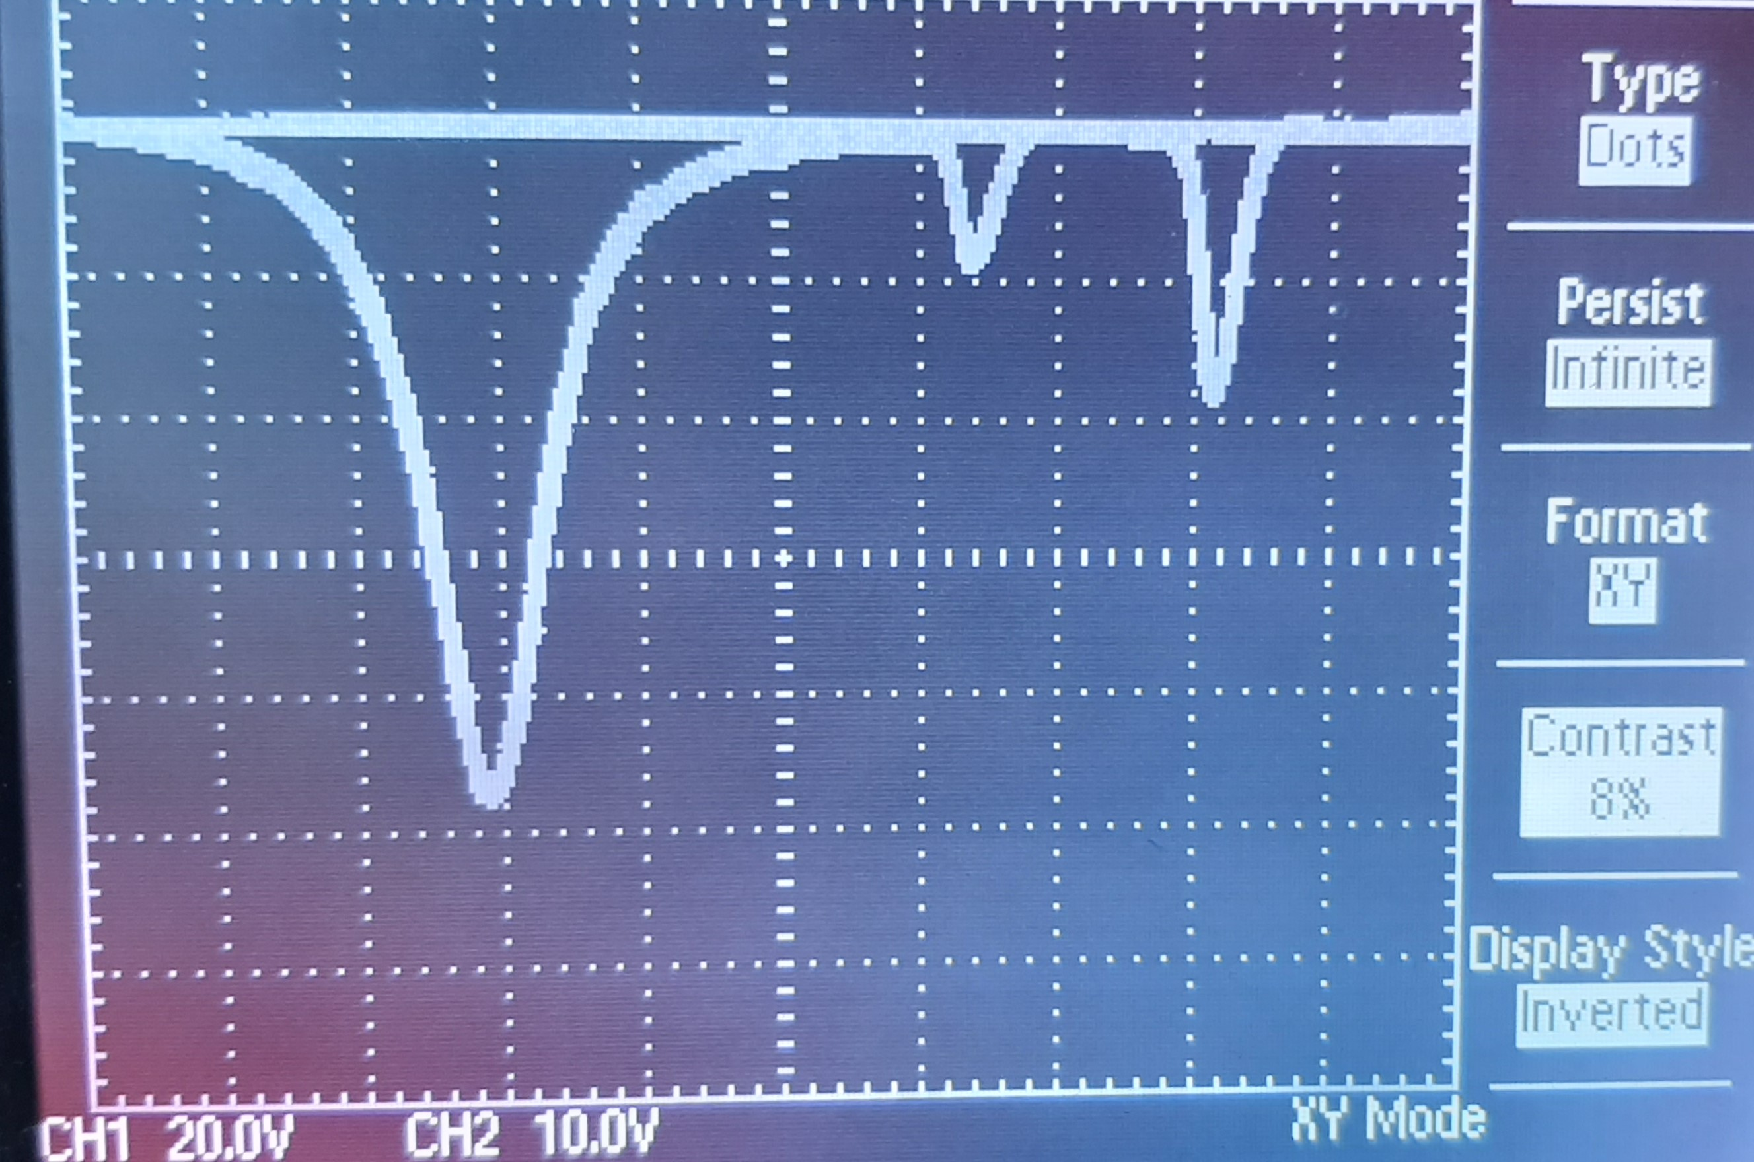
\includegraphics[width=0.8\textwidth]{Messdaten/v21_oszi.pdf}
    \caption{Fotografie des Oszilloskops. Auf der x-Achse des Oszilloskop ist die Stärke des Magnetfeldes zu sehen und auf der y-Achse die Transparenz der Rubidiumprobe.}
    \label{fig:bildoszi}
\end{figure}

Die Transparenz ist von der Menge an Atomen abhängig, die durch das Licht angeregt werden können.
Das nullte Minimum (links) $B = 0$ ist der Nulldurchgang.
Alle Rubidiumatome können angeregt werden.
Das erste Minimum (Mitte) ist Rb-87 und das zweite Minimum (rechts) ist Rb-85.
Um die maximale Absorption abzuschätzen, werden die Pixel zwischen der Basis eines Peaks und der Spitze gezählt.
Für Rb-87 werden 24 Pixel und für Rb-85 49 Pixel gezählt.
Das ergibt ein Verhältnis von $32,88\, \%$ für Rb-87 und $67,12 \, \% $ für Rb-85.

\subsection{Abschätzung des Quadratischen Zeeman-Effekts}

Es wird die Größenordnung des quadratischen Zeeman-Effekts abgeschätzt, 
dabei werden als Werte für die Hyperfeinstrukturaufspaltung des Grundzustandes bei 87-Rb: $4,53 \cdot 10^{-24} \, \unit{\joule} $ und $2,01 \cdot 10^{-24} \, \unit{\joule}$ bei  85-Rb  gewählt \cite{v21}.
Die Energie des quadratischen Zeeman-Effekts kann mit \eqref{eq:QuadZee} berechnet werden.
Es wird der Wert des größten gemessenen Magnetfeldes verwendet. Aus den Auswahlregeln ergeben sich die Quantenzahl $m_\text{F} = 2$ für Rb-87 und $m_\text{F} = 3$ für Rb-85.
Daraus werden 
\begin{align*}
    E_{\text{Quad},1} &= \left(7,78  \pm 0,05 \right)   \cdot 10^{-28} \, \unit{\joule} \, \text{und} \\
    E_{\text{Quad},2} &= \left(7,352 \pm 0,010 \right) \cdot 10^{-28} \, \unit{\joule}
\end{align*}
berechnet.